
\documentclass[submit,techreq]{ipsj}
%\documentclass[submit,draft]{ipsj}


\usepackage[dvips]{graphicx}
\usepackage{latexsym}

\def\Underline{\setbox0\hbox\bgroup\let\\\endUnderline}
\def\endUnderline{\vphantom{y}\egroup\smash{\underline{\box0}}\\}
\def\|{\verb|}

\setcounter{巻数}{53}
\setcounter{号数}{10}
\setcounter{page}{1}

\受付{2011}{11}{4}
%\再受付{2011}{7}{16}   %省略可能
%\再再受付{2011}{7}{20} %省略可能
\採録{2011}{12}{1}

\begin{document}


\title{語の出現パターンと意味関係分析を用いた\\
Webからのタスク検索}

\etitle{Subtask search}

\affiliate{IPSJ}{情報処理学会\\
IPSJ,Chiyoda,Tokyo 101--0062,Japan}


\paffiliate{KU}{京都大学\\
Kyoto Uniersity}



\author{加藤 龍}{Ryo Kato}{IKU}[r.kato@dl.kuis.kyoto-u.ac.jp]
\author{大島 裕明}{Hiroaki Ohshima}{IPSJ}[ohshima@dl.kuis.kyoto-u.ac.jp]
\author{山本 岳洋}{Takehiro Yamamoto}{IPSJ,KU}[yamamot@dl.kuis.kyoto-u.ac.jp]
\author{田中 克己}{Katsumi Tanaka}{IPSJ,KU}[ktanaka@i.kyoto-u.ac.jp]
\author{加藤 誠}{Makoto P. Kato}{IPSJ,KU}[kato@dl.kuis.kyoto-u.ac.jp]

\begin{abstract}
本研究では,クエリとしてタスクが与えられた際に,そのタスクを達成するために必要なサブタスク群をWebから発見する手法を提案する. 提案手法では,動詞の含意関係や逆意関係にもとづいたルールによりクエリの変換を行う. 変換したクエリでWeb検索を行う. 得られたページから,タスク特有の言語パターンを用いて,サブタスク候補となるフレーズを発見する. 
\end{abstract}

\begin{jkeyword}
タスク検索
\end{jkeyword}

\begin{eabstract}
This study is about subtask search. We propose a new method to find subtasks from the Internet. When a query is given, our method find subtasks which are needed to acomplish the task represented by the query. In our method, the system convert the query according to relationships of words such as the relationship of includingness and contradiction. The system find phrases from the pages which are listed up by our method. After that, we use language patterns which are specified in tasks to find phrases which are possible to be correct subtask.
\end{eabstract}

\begin{ekeyword}
Task search
\end{ekeyword}

\maketitle

%1
\section{動機}

誕生以来,Webには多様な資料が集積され続けている. 情報をどう走査,発見し,取捨選択するか,様々な方向からのアプローチがなされている. 
現在,いくつもの検索エンジンが実用化され,Webを舞台に情報発見や集約を行っている. だが,Webにおける情報検索は,いまだ多くの問題を抱えている. 
そのうちの一つとして,目的を達成する手段を発見したいとき,できるだけ多くの方法を探そうとしても意外と見つけられないことがあげられる.


なにかを成し遂げたいが,どうすれば成功するかわからないとき,Web検索を使って実現方法を考える行為がよく行われている. たとえば「花粉症対策をする方法」をクエリに検索することで,立体マスクをつける」や「アレロック錠剤を飲む」を発見することができる. だが,そうして発見できた「花粉対策をする方法」を採用すべきなのか,簡単にはわからない. まだ発見できていない「花粉対策をする方法」のほうがよいかもしれないからだ.


こうした状況では,多くのユーザーは「タスクを遂行するためにどんな方法があるか」をできるだけ多く発見するサブタスク検索を求める. 多様な答えが得られた段階で,初めて,安心して各方法を比較したり,自分にとって最適な方法を考えることができるようになる.

サブタスク検索の例を説明する.たとえば「花粉症対策をする」というクエリを入力すると,出力として


\begin{itemize}
\item \|立体マスクをつける|
\item \|アレロック錠剤を飲む|
\item \|医師の診断を受ける|
\item \|植物に近寄らない|
\end{itemize}


といったように,複数の異なった選択肢を複数発見する.これがサブタスク検索の例である. このように,できるだけ多くの手法を探そうとする検索は現在の一般的な検索エンジンでは困難である. 花粉症対策の方法は非常に多様であり,高くランクづけされたページであっても花粉症対策の方法のごく一部を含んでいるにすぎない. また高くランクづけされたページ同士は内容が重複していることが多く,高ランクのページを見て回っても,発見できる花粉症対策の方法の数は増えない。

このようなサブタスク検索が実用的なレベルに達すれば、\figref{fig:future_app}のように、 現在の検索エンジンが実装しているサジェスト機能にサブタスク検索を組み込むといった応用が考えられる。

\begin{figure}[tb]
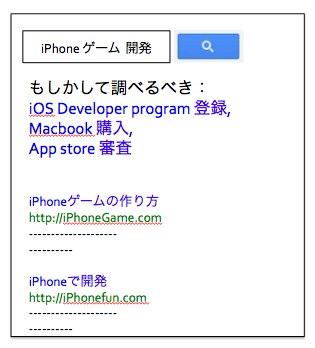
\includegraphics[width=6cm, bb=0 0 240 400]{future_app.jpg}
\caption{アプリケーションの例}
\ecaption{Application.}
\label{fig:future_app}
\end{figure}

サブタスク検索は、タスクを遂行する方法が複数あり、どれがベストかわからない状態で役割を果たす。\figref{fig:future_app}は、まさしくその一例である。クエリに「iPhone ゲーム 開発」と入力した結果、通常のWeb検索であってもiPhoneゲームの作り方についてのWebページを非常に多量に発見できる。しかし、通常の検索のみでは人気の高いページだけが上位にランクづけされてしまう。そのため、iPhoneのゲームを開発するためにやるべき行動をすべて網羅できない。このとき、「App storeの審査を受ける」といった、やらねばならないことだが、上位ページではあまり言及されないタスクに気づかない、といった問題が発生しうる。こうした状況でサブタスク検索を行うことで、iPhoneのゲームを開発するために必要なタスクがすべて明らかになり、タスク遂行のためのロードマップを描きやすくなる。

逆にサブタスク検索が不得意なこととして、遂行する方法がひとつのタスクがある。たとえばすでに手元に本があるとき「手元の本を読む」というタスクを遂行する方法はひとつである。

サブタスク検索が有効に働くのは、多くの、時間のかかる作業をせねばならないときである。


タスク検索は、Web検索のなかでもかなりの割合を占めている。サブタスク検索を実現することは、Webでの検索体験を向上させる点で非常に有意義である。

以下、本稿では可能な限り多様な方法をWebから発見する手法を提案し,評価する。


%2
\section{関連研究}

タスク検索に関する研究として、以下のものがある。

\begin{itemize}
\item \|ゴールにもとづいたクエリのクラスタリング|
\item \|タスクにもとづいた検索行動の推移|
\item \|タスクに適したウェブサイトを発見するサービス検索|
\end{itemize}

山本らの研究\cite{yamatake}において,スポンサードサーチ広告を用いたクエリクラスタリングが試みられている。スポンサードサーチ広告は、できるだけ多くのユーザーの注目を集めることを目的としている。それも、広告の商品を使いたいだろうユーザーの注目を集めようとしている。こうした理由から、スポンサードサーチのスニペットやタイトルは、クエリに呼応した工夫がなされたものとなる。つまり、「クエリが意味するタスクを達成するために、広告の商品が必要になる」ことが、スニペットやタイトルを読むと理解できるような工夫がなされる。逆にいえば、タスクを表現するクエリを入力したときに出力されるスポンサードサーチ結果は、タスクを遂行するのに必要なものになる。本研究においてもこのアイディアを利用している。

ほかに、タスク遂行のための,複雑な検索の手順を研究したものとしてHassanらの\cite{hassan}がある。タスクを遂行するのに、一度だけの検索では不十分なことが多い。タスクを達成するためには、通常、何度も検索を試行しなければならない。\cite{hassan}は、こうした複数の検索においてのユーザーの行動を研究したものである。


田麦らによるタスク遂行のためショッピングサイトなどサービスを提供するページを発見する研究\cite{tamugi}がある。「中古ギターを売る」といったタスクを遂行する際、「中古ギター 売却」というクエリで検索を行うよりも、「中古ギター 買い取り」というように、サービス提供者がわの視点での行動にクエリ変換したほうが、タスク遂行に適したページを発見しやすいことがある。\cite{tamugi}は、サービス提供者とサービス享受者の視点を軸にしたタスク検索研究といえる。


%3
\section{タスク関係の概要}
本章ではタスクとゴールの概念を述べ、タスクを遂行する行動がどのようにモデル化されるかを説明する。


%3.1
\subsection{ゴールとアクション}
ある目的を達成するためにどのような順番でどのような行動を取るか考察する際,タスク,ゴール,アクションといった用語の定義が必要となる。
本稿ではゴールとアクションを以下のように定義する。

\begin{itemize}
\item \|ゴールとは,目的の一部または全部を達成した状態である|
\item \|アクションとは,ある状態から別の状態に移行する行為である|
\end{itemize}

ゴールとアクションを図示すると\figref{fig:action_goal}のようになる。「花粉症対策している状態」がゴールであり、「花粉症対策をしていない状態」から「花粉症対策している状態」に移行する行為がアクションである。\figref{fig:action_goal}では、ひとつのアクションでゴールに移行しているが、実際はひとつのアクションだけでゴールに移行できるとは限らない。多段階でのゴール移行を表現すると、\figref{fig:sub_goal}のようになる。

\begin{figure}[tb]
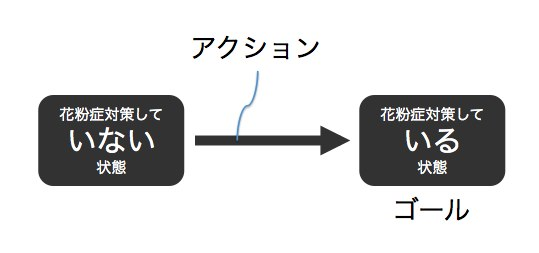
\includegraphics[width=6cm, bb=0 0 400 300]{action_goal.jpg}
\caption{アクションとゴールの例}
\ecaption{Action.}
\label{fig:action_goal}
\end{figure}

\figref{fig:sub_goal}はサブゴールという概念を表現している。「花粉症対策をしていない状態」から「花粉症対策している状態」に移行する間に、別の「花粉症について調べている状態」というものを経由している。


\begin{figure}[tb]
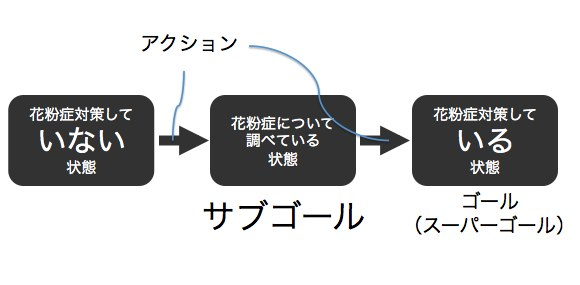
\includegraphics[width=6cm, bb=0 0 450 300]{sub_goal.jpg}
\caption{サブゴールの例}
\ecaption{Subgoal}
\label{fig:sub_goal}
\end{figure}



\figref{fig:many_sub_goals}に図示したように、ひとつのゴール(スーパーゴール)にサブゴールは複数ありえる。スーパーゴールとサブゴールの関係は、後述のスーパータスクとサブタスクの関係と同様に、相対的なものである。サブゴールからサブゴールへの移行もアクションのひとつである。



\begin{figure}[tb]
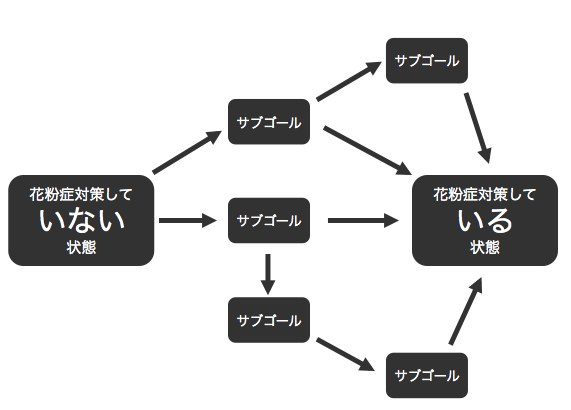
\includegraphics[width=6cm, bb=0 0 450 400]{many_sub_goals.jpg}
\caption{複数のサブゴール}
\ecaption{Many sub goals}
\label{fig:many_sub_goals}
\end{figure}



%3.2
\subsection{タスクとサブタスク、スーパータスク}
\label{task_and_goal}


次に、タスクの定義を説明する。

\begin{itemize}

\item \|タスクとは,遂行すると,目的の一部あるいは全部を達成したことになるアクションである|
\item \|サブタスクとは,タスク同士の関係に着目したとき,「遂行するともう一方のタスクの一部を遂行したことになる行動」である. このとき「もう一方のタスク」はスーパータスクである|
\end{itemize}

つまり,なんらかのゴールに至るアクションがタスクといえる。ゴールとタスクの関係を\figref{fig:action_task}に図示する。状態を変化させる行為すべてがアクションであるが、アクションのうち、目的の一部あるいは全部を達成したものだけがタスクである。


\begin{figure}[tb]
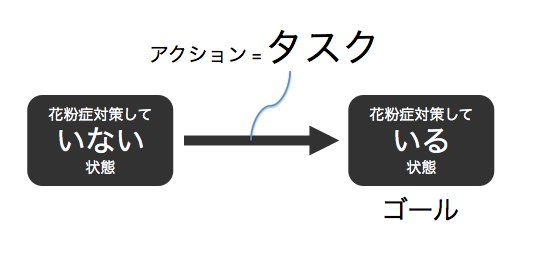
\includegraphics[width=6cm, bb=0 0 400 300]{action_task.jpg}
\caption{タスクの例}
\ecaption{Action Task.}
\label{fig:action_task}
\end{figure}


タスクもゴールと同様、複数の階層に分割できる。\figref{fig:super_task}にスーパータスクとサブタスクの関係を図示する。

\begin{figure}[tb]
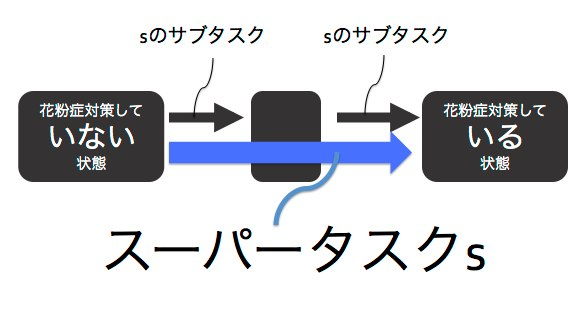
\includegraphics[width=6cm, bb=0 0 400 300]{super_task.jpg}
\caption{スーパータスクの例}
\ecaption{Supertask.}
\label{fig:super_task}
\end{figure}

このタスクを分割すると、まず「花粉症対策していない状態」から「花粉症対策している状態」に移行するタスクをスーパータスクとみなし、「花粉症対策していない状態」から別の何らかの状態への移行がひとつめのサブタスク、何らかの状態から「花粉症対策している状態」への移行がふたつめのサブタスクだとみなせる。

%3.3
\subsection{木構造によるタスク分割}

上記のタスクの説明は状態遷移図によるタスク構造のモデル化である。表現を変え、タスクをand-or木構造と見なすこともできる. 実際はタスクを遂行する順序やあるタスクを遂行できて初めて遂行可能になるタスクなども存在するため,and-or木構造よりももっと複雑な構造となる.


\begin{figure}[tb]
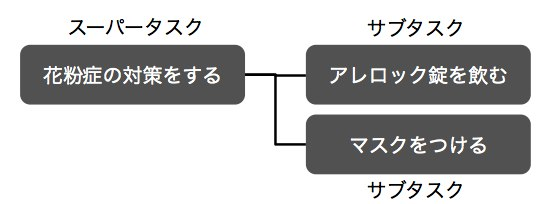
\includegraphics[width=6cm, bb=0 0 400 272]{super_sub.jpg}
\caption{スーパータスクとサブタスクの関係}
\ecaption{Relationships of super task and sub tasks}
\label{fig:super_sub}
\end{figure}

\figref{fig:super_sub}に示すように、サブタスクとスーパータスクは相対的な関係である. あるサブタスクは,別のタスクをサブタスクだとして見ればスーパータスクにあたることもある.

例えば「花粉症対策をする」がスーパータスクだと仮定すると,サブタスクとして「アレロック錠を飲む」,「マスクをつける」といったタスクがあげられる. ここで一段階視点を下げて「アレロック錠を飲む」をスーパータスクと捉えた場合,「診断を受ける」,「薬局を探す」といった行動がサブタスクとなる. 逆の順番でいえば,「薬局に行く」というサブタスクから見たとき「アレロック錠を飲む」はスーパータスクだが,「アレロック錠を飲む」をサブタスクとした場合スーパータスクは「花粉症対策をする」となる.

\begin{figure}[tb]
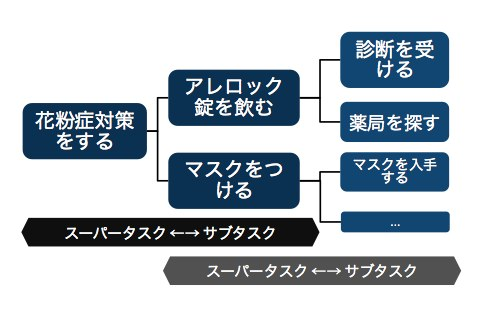
\includegraphics[width=6cm, bb=0 0 350 319]{super_sub_sub.jpg}
\caption{スーパータスクとサブタスクの多重関係}
\ecaption{Multiple relationships of super task and sub tasks}
\label{fig:super_sub_sub}
\end{figure}


ここで注意してほしい点がある. 「花粉症対策をする」のサブタスクとして「薬局に行く」もありうる. 二段階,三段階下のタスクであってもそれはサブタスクなのである. 逆に,「薬局に行く」のスーパータスクとして「花粉症対策をする」がある. つまり,複数段階の連続的な関係と,サブ・スーパーの一段階の関係は両立できる。多重のスーパータスクーサブタスク関係を\figref{fig:super_sub_sub}に図示する。サブタスクのサブタスクのサブタスク、といったように、タスク分割は複数段階行えることが多い。

ただし、それ以上分割できないタスクが存在し、これをアトミックタスクと呼ぶ。アトミックタスクは空の状態から何らかの状態に移行するアクションである。


ある目的を達成するために行動を起こす際,どのような手順で状態が変異するのか整理をする. まず最終的な目的として「花粉対策をする」というタスクがあるとする. これは「花粉症対策をした」というゴールと等価である.

ユーザーは「花粉症対策をしていない」という状態から「花粉症対策をした」という状態に遷移するために必要なアクションを発見しようとする.

「花粉症対策をする」というタスクを遂行する方法はいくつも存在する. 「アレロック錠を飲む」,「マスクをつける」,「医師の診断を受ける」,「薬局に行く」これらすべてが「花粉対策をする」のサブタスクである.



%4
\section{サブタスク検索の手法}
本章では、スポンサードサーチを利用したサブタスク検索を提案する。

%4.1
\subsection{サブタスク検索における入力と出力}
本稿で扱うサブタスク検索の入力と出力を述べる。
ユーザーは「(動詞)」または「(名詞)(助詞)(動詞)」というクエリを入力する。一例として「花粉症の対策をしたい」という意図でタスク検索を行う場合、「花粉症対策をする」といったクエリが考えられる。入力の例として、以下のものがあげられる。

\begin{itemize}
\item \|花粉症対策をする|
\item \|部屋を掃除する|
\item \|二日酔いを覚ます|
\item \|ダイエットする|
\item \|快眠する|
\item \|おいしいコーヒーを淹れる|
\end{itemize}

以上の例はタスクを動詞として表現したものであるが、実際にはタスクの表現としては動詞以外のものも考えられる。「花粉症対策」「掃除」「快眠」といったものがその例である。

さらに、タスクの表現として「花粉症対策をした状態」つまりゴールをそのまま使うこともできる。ゴールとタスクは別のものであるが、クエリとして用いる場合、どちらも同様のものと見なせる。ゴールとタスクの違いは前述の通りであるが、サブタスク検索においては、違いを無視して利用できるのである。

\figref{fig:goal_can_be_task}に図示したように、初期状態を持てないことを除けば、ゴールもタスクとして扱える。本来のタスクとは、状態が目的の状態に変化するアクションであるので、ゴールも初期状態を考えなければ「状態に変化する」というアクションと同様に、クエリに使える。整理すると、まずタスクは以下のようなものである。

\begin{itemize}
\item \|タスクは初期状態とゴールが与えられれば成立する|
\item \|タスクはアクションである|
\end{itemize}

そしてゴールは以下のようなものである。

\begin{itemize}
\item \|ゴールには初期状態が与えられない。不要である。|
\item \|ゴールは状態である|
\end{itemize}


以上の特徴から、タスクとゴールは明らかに違うものであるが、ゴールを「初期状態のないタスク」として扱うことができる。

しかし本稿ではゴールによるタスク表現は扱わない。あくまで「(動詞)」または「(名詞)(助詞)(動詞)」のみをタスクとして扱う。


\begin{figure}[tb]
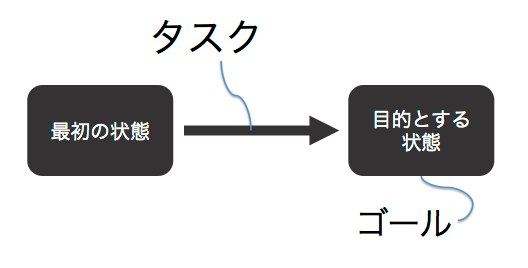
\includegraphics[width=6cm, bb=0 0 350 319]{goal_can_be_task.jpg}
\caption{ゴールがタスク表現としても扱える}
\ecaption{Multiple relationships of super task and sub tasks}
\label{fig:goal_can_be_task}
\end{figure}

「花粉症対策をする」をクエリとした場合の、サブタスク検索の出力を例示する。

\begin{itemize}
\item \|立体マスクをつける|
\item \|アレロック錠剤を飲む|
\item \|医師の診断を受ける|
\item \|植物に近寄らない|
\end{itemize}

以上のように、クエリをスーパータスクとした場合のサブタスクである「(名詞)(助詞)(動詞)」の文章が出力される。

%4.2
\subsection{提案手法}
本稿ではスポンサードサーチを用いたサブタスク検索を提案する。スポンサードサーチとは、ユーザーの入力した検索クエリに対応した広告を表示するシステムである。GoogleやBing, Yahoo!など、多くのサーチエンジンがスポンサードサーチを提供している。スポンサードサーチによりユーザーは自分の入力したクエリに適した広告ページを見ることができ、広告主は広告の商品に適したユーザーにアプローチすることができる。


%4.2.1
\subsubsection{スポンサードサーチを用いたサブタスク検索}
スポンサードサーチを利用して、以下のような手法でサブタスク検索を実現できる。

\begin{enumerate}
\item \|言語パターンに基づいてクエリを変換する|
\item \|変換したクエリをもとにスポンサードサーチを行う|
\item \|得られたページ情報からサブタスクを抽出する|
\end{enumerate}

本稿は、このような手法によるサブタスク検索を提案する。最初の手順である言語パターンによるクエリ変換は、単語間の上位語、下位語などのエンテイルメント関係に着目して行う。


スポンサードサーチに着目した理由を述べる。スポンサードサーチには、商品を購買しそうなユーザーの目に留まるように多くの工夫がなされている。具体的には、商品に対応したクエリを入力したときに広告が表示されるように設定されており、スニペットの文章は商品のニーズを端的に表現している。これは\cite{yamatake}が指摘した通りである。このような特徴を利用すれば、サブタスク検索に使えると我々は考えている。

ユーザーが目的とするゴールに到達するために、スポンサードサーチに広告を出している企業の商品を使うことは有効な場合が多い。本稿の\ref{sec:evaluate}で用いた「花粉症対策をする」といったクエリであれば、「立体マスクをつける」「花粉症の薬を飲む」といったサブタスクはどちらも商品を使用することで達成できる。

%4.2.2
\subsubsection{ショッピングサイトを用いたサブタスク検索}
本研究ではショッピングサイトを利用したサブタスク検索を提案する。

ショッピングサイトに着目した理由として、以下の理由がある。

\begin{itemize}
\item \|タスク遂行の手法に商品を使うものが多い|
\item \|ショッピングサイトには商品のニーズを端的に説明する文章が載っている|
\item \|タスク遂行の結果が、商品を利用したユーザーによるレビューとして表現されている場合がある|
\item \|商品がカテゴリに分類されており、上位語・下位語の概念を利用したサブタスク発見ができる|
\end{itemize}


ショッピングサイト中の文章には、いくつかの特徴がある。商品を求める可能性のあるユーザーの目にとどまりやすいような工夫がなされているのは、スポンサードサーチと同様である。さらにショッピングサイトには、スポンサードサーチにはない、サブタスク検索に活用できる利点がある。

レビューや商品のカテゴライズなど、明確な目的を持った文章が、一定の分量で存在することである。これらの文は


問題点として、一部の商品しかショッピングサイトには載らないことがあげられる。たとえば「部屋の掃除をする」には「家事代行に依頼する」というサブタスクがある。しかし一般的なショッピングサイトは家事代行サービスを扱っていない。

あらゆる商品を並列に扱うショッピングサイトは存在しない。そのため、より多くの種類の、なんらかの商品を使うサブタスクを発見しようとするなら、複数のショッピングサイトを併用する必要がある。

ショッピングサイトを用いたサブタスク検索の手順を以下に述べる。

\begin{enumerate}
\item \|言語パターンに基づいてクエリを変換する|
\item \|変換したクエリをもとにショッピングサイト内で検索を行う|
\item \|得られたページ情報からサブタスクを抽出する|
\end{enumerate}


%5章
\section{評価}
\label{sec:evaluate}
本章では、提案手法によりサブタスク検索を行い、その性能を適合率と発見数により評価する。

%5.1
\subsection{実験の手法}
提案手法とベースライン手法を述べる。

%5.1.1
\subsubsection{スポンサードサーチを利用したサブタスク検索}

提案手法では、Yahoo! Japanが提供するスポンサードサーチ\footnote{http://search.yahoo.co.jp/search/ss}を利用してサブタスク発見を試みる。言語パターンよりサブタスク表現を探す際、形態素解析にMeCab\footnote{https://code.google.com/p/mecab/}を用いる。提案手法の処理を順番にすると以下のようになる。

\begin{enumerate}
\item \|クエリを形態素解析して名詞と動詞を抽出する|
\item \|名詞と動詞をキーワードにした新たなクエリを作成する|
\item \|新たなクエリでYahoo! Japanのスポンサードサーチを行う|
\item \|最大15件のページとタイトル、スニペットを取得する|
\item \|発見したスニペットにMecabで形態素解析を行い、動詞とサ変接続名詞を取得する|
\item \|取得した単語のうち、出現頻度の高いもののみをピックアップする|
\item \|動詞とサ変接続名詞をサブタスクとして適した「〜〜する」といった形にする|
\end{enumerate}

以上の手順でサブタスクを発見する。

%5.1.2
\subsubsection{ショッピングサイトを利用したサブタスク検索}
もうひとつの提案手法について詳細に述べる。ショッピングサイトを利用したサブタスク検索を我々は提案する。本稿ではAmazon Product Advertising API\footnote{https://affiliate.amazon.co.jp/gp/advertising/api/detail/main.html}を利用して、Amazonページ内よりサブタスクを発見する。具体的な手法を述べる。

\begin{enumerate}
\item \|クエリを形態素解析して名詞と動詞を抽出する|
\item \|名詞と動詞をキーワードにした新たなクエリを作成する|
\item \|新たなクエリでAmazon中で検索を行う|
\item \|適した商品ページを取得する|
\item \|商品の使用がサブタスクとして適しているかフィルタリングを行う|
\end{enumerate}



%5.1.3
\subsubsection{ベースライン手法}

またベースラインとして、単純な言語パターンを用いてサブタスク検索を行うシステムを使う。

ベースラインは上位にランクづけされたページをスクリプティングすることでサブタスクを発見する。上位にランクづけされたページ内から、タスクに使われることの多い「使う」「おすすめ」「〜〜してください」「〜〜しないでください」といった単語を検索し、その前後の文章をサブタスクとする。

\begin{enumerate}
\item \|クエリを形態素解析して名詞と動詞を抽出する|
\item \|名詞と動詞をキーワードにした新たなクエリを作成する|
\item \|Google Cusom Search APIを使い,新たなクエリでWeb検索する|
\item \|上位100件のページを取得する|
\item \|ページ内から「使う」「おすすめ」といったタスクに使われる可能性の高い単語を含む文章を発見する|
\item \|発見した文章に係り受け解析を行い、サブタスクとして適した表現に変換する|

\end{enumerate}

以上の手順で,タスクと推測できる文を発見する。
ベースラインの問題として、ノイズが非常に多く含まれることがあげられる。現実のHTML中にはコメント内に「この行は削除しないでください」といった文章を持つことや、「ボタンを押して下さい」といった明らかにサブタスクではない文を持つことがある。これらのノイズをフィルタリングする必要があるが、ノイズ除去の有効な手法は発見できていない。

将来の課題として、このノイズ除去があげられる。機械学習を用いたノイズ除去や、自然言語処理による手法が考えられる。係り受け解析を行い、「(名詞)(助詞)(動詞)」のパターンに準じたサブタスク候補だけを採用する、


%5.1.3
\subsubsection{実験に用いるクエリ}

実験に用いるクエリとして、サブタスク検索に使われるだろう以下の一般的なクエリを使用する。

\begin{itemize}
\item \|花粉症対策をする|
\item \|部屋を掃除する|
\item \|二日酔いを覚ます|
\item \|ダイエットする|
\item \|快眠する|
\item \|おいしいコーヒーを淹れる|
\end{itemize}


以上のクエリから、サブタスクを探す。
理想的なサブタスクとしては、たとえば「部屋を掃除する」をクエリとした場合、

\begin{itemize}
\item \|掃除機をかける|
\item \|パナソニックの掃除機を買う|
\item \|家事代行に依頼する|
\item \|友達に掃除を頼む|
\item \|ルンバを使う|
\item \|お茶の出がらしをまく|
\end{itemize}

といったサブタスクが出力されれば理想的である。ここで注意していただきたいことがある。「掃除機をかける」と「パナソニックの掃除機を買う」は並列したタスクではなく、「パナソニックの掃除機を買って、それから掃除機をかける」という連続的関係にあるタスクかもしれない。しかし本研究では連続したタスクであっても、別個のタスクとして扱う。よって、「掃除機をかける」と「パナソニックの掃除機を買う」は別のタスクだと判断する。


%5.1.4
\subsubsection{評価手法}
適合率と発見数で評価を行う。スーパータスクをクエリとして検索を行い、発見できたサブタスク候補のうち、実際にサブタスクであったものの割合を適合率、実際にサブタスクであったものの個数を発見数とする。サブタスク候補がサブタスクとして正解であったかどうかは、人の手で判断する。判断基準を説明する。例えば、「花粉症対策をする」というクエリを入力したとして、

\begin{itemize}
\item \|乾燥機やエアコンで代用する|
\item \|加湿器を使う|
\item \|冷えを解消する|
\item \|ほどほどにする|
\item \|花粉と触れる部位を減らす|
\item \|寄生虫を飼う|
\item \|自分の体調に合えば使う|
\item \|汁を摂って綿棒で鼻内の粘膜に塗る|
\item \|薬剤師に相談する|
\item \|鼻の下はしっかり洗う|
\item \|ノウハウのメモをとる|
\item \|ラジオ体操をする|
\end{itemize}

以上の出力が返ってきたとする。このうち、実際のサブタスクだと判断できるものは以下の通りである。

\begin{itemize}
\item \|加湿器を使う|
\item \|花粉と触れる部位を減らす|
\item \|寄生虫を飼う|
\item \|薬剤師に相談する|
\item \|鼻の下はしっかり洗う|
\item \|冷えを解消する|
\item \|ラジオ体操をする|
\end{itemize}


サブタスクではないと判断できるものは以下の通りである。

\begin{itemize}
\item \|乾燥機やエアコンで代用する|
\item \|ほどほどにする|
\item \|自分の体調に合えば使う|
\item \|汁を摂って綿棒で鼻内の粘膜に塗る|
\item \|ノウハウのメモをとる|
\end{itemize}


判断の基準として「それ単体で、遂行すべきサブタスクが何なのか明確であること」があげられる。「乾燥機やエアコンで代用する」では何の代用をするのかわからず、明確ではない。だが「ラジオ体操をする」は、判断が難しい。「ラジオ体操をする」ことが花粉症対策として有効であるかどうか、簡単には結論を下せない。世界のどこかに「花粉症対策にはラジオ体操がよい」と考える人々がおり、彼らの間ではラジオ体操は花粉症対策として一般的かもしれないからだ。

こういった、判断しにくいサブタスク候補に対しては、「実際にサブタスクとして遂行している人が存在しているか」が基準となる。サブタスク候補を発見したWebページを訪問し、サブタスク候補の文章が「スーパータスク遂行にはサブタスク候補の遂行が必要」と主張しているかで判断する。明らかに、サブタスクだと意図していない文脈であった場合、サブタスクではないと判断できる。


\begin{figure}[tb]
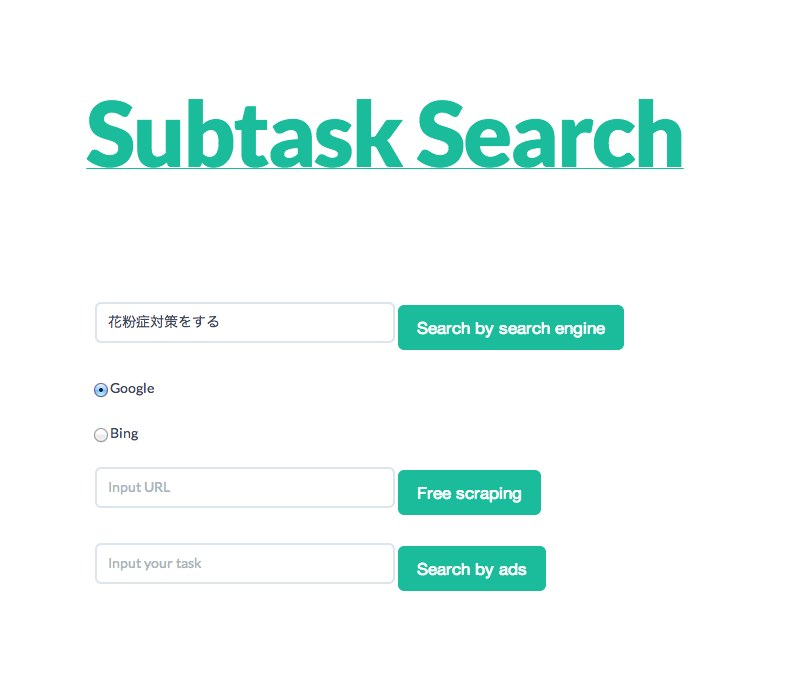
\includegraphics[width=6cm, bb=0 0 550 719]{base_line1.jpg}
\caption{ベースライン}
\ecaption{Multiple relationships of super task and sub tasks}
\label{fig:single}
\end{figure}


%5.2
\subsection{実験の結果}

結果を\figref{fig:super_sub}に示す。
ベースラインの結果ページは\figref{fig:baseline_result}のようになった。



\begin{figure}[tb]
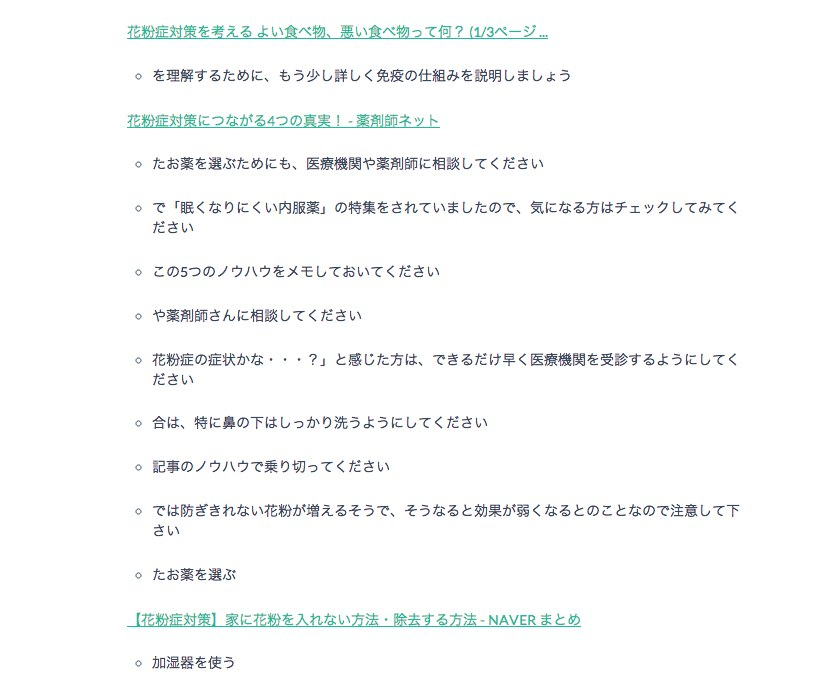
\includegraphics[width=6cm, bb=0 0 550 719]{base_line3.jpg}
\caption{ベースラインの結果}
\ecaption{Multiple relationships of super task and sub tasks}
\label{fig:baseline_result}
\end{figure}




\begin{table}[tb] 
\caption{花粉症対策の方法タスク検索} 
\ecaption{An Example of Table.}
\label{tab:result}
\hbox to\hsize{\hfil
\begin{tabular}{l|lll}\hline\hline
& 発見数 & 正解数 & 正解率 \\\hline
ベースライン &	131 & item 2,1 & ---\\
row4 &	item 1,4 & item 2,4 & item 3,4 \\\hline
\end{tabular}\hfil}
\end{table}



%6
\section{考察}


\figref{fig:baseline_result}のように、ベースラインの手法では,「医療機関や薬剤師に相談する」「加湿器を使う」「花粉症の市販薬を選ぶ」といったタスクを発見できる.しかし「むずむずするときに飲んでみてください」といったタスクの断片や、そもそもタスクではない「設定してください」といった文も発見してしまう。単純に言語パターンを用いるだけではタスクを表現する文章を発見しにくく、発見できた文章がタスクかどうかのフィルタリングも簡単ではないことが明らかとなった。

提案手法は提案は15件までしかスポンサードサーチ結果を取得できず、十分な量のスニペットを得ることができなかった。もっと多くのスポンサードサーチ結果を取得できれば、より性能の高いサブタスク検索を実現できると期待できる。

またスニペットは商品のニーズを端的に表したものではあるが、必ずしもサブタスクをそのまま表現しているわけではない。これはスポンサードサーチのスニペットが広告文章であることが原因である。たとえば「二日酔いを覚ます」というタスクに対し、スポンサードサーチを用いたサブタスク検索では「添加する」「サポートする」といったノイズを出力する例があった。「添加」や「サポート」は、「二日酔いに疲れた脳に効く成分を添加」や「二日酔いのあなたをサポートする」といった文面から、サブタスクとして抽出された結果である。これらは商品のアピールとしては有効であるが、サブタスクではない。

広告スニペットではなく、サブタスクそのものを表現する「(商品名)を使う」といったサブタスクを出力に利用することで、適合率を高めることが期待できる。


%7
\section{結論}
本稿では、スポンサードサーチに着目し、サブタスク検索を行った。スポンサードサーチの広告意図を利用してのサブタスク検索を提案し、評価した。本研究の結果を整理すると以下のようになる。


\begin{itemize}
\item \|ゴール、タスクを定義した。|
\item \|スポンサードサーチを利用したサブタスク検索を提案した。|
\item \|提案手法は、サブタスク発見のために有用であることを示した。|
\end{itemize}

サブタスク検索を必要とするユーザーは多く、活用の状況がいくつか考えられる。今後、サブタスク検索が役割を果たす。

将来の研究課題として、サブタスク候補からのノイズ除去、より広範なサブタスク発見があげられる。本稿ではスポンサードサーチとショッピングサイトを利用したサブタスク発見を行った。これは、広告やショッピングサイトにおいてmユーザーのニーズに適した商品、商品に適した文章を用いて商品をアピールする工夫がなされていることを利用したものである。しかし、サブタスクを発見できるWebページはこれらショッピングサイト、スポンサードサーチに限ったものではない。より多くのサブタスクを発見するために、別の点に着目した検索が必要になるだろう。


\begin{thebibliography}{10}


\bibitem{yamatake}
The Widwom of Advertisers: Mining Subgoals via Query Clustering
\urlj{http://research.microsoft.com/en-us/people/tesakai/cikm2012yamamoto.pdf}
(2012.11.02).

\bibitem{hassan}
Task Tours: Helping Users Tackle Complex Search Tasks:
Ahmed Hassan,Ryen W. White
\urlj{http://research.microsoft.com/pubs/178868/HassanCIKM2012.pdf}

\bibitem{tamugi}
Tamugi search:
\urlj{http://somewhere.pdf}




\end{thebibliography}



\begin{biography}
\profile{s}{加藤 龍}{1988年生.2012年京都大学農学部卒. 2012年同大学院情報学研究科入学}
%
\end{biography}



\end{document}
